\documentclass[12pt,letterpaper]{hmcpset}
\usepackage[margin=1in]{geometry}
\usepackage{graphicx}
\usepackage{amsmath,amssymb}
\usepackage{enumerate}
\usepackage{hyperref}
\usepackage{parskip}

% Theorems
\usepackage{amsthm}
\renewcommand\qedsymbol{$\blacksquare$}
\makeatletter
\@ifclassloaded{article}{
    \newtheorem{definition}{Definition}[section]
    \newtheorem{example}{Example}[section]
    \newtheorem{theorem}{Theorem}[section]
    \newtheorem{corollary}{Corollary}[theorem]
    \newtheorem{lemma}{Lemma}[theorem]
}{
}
\makeatother

% Random Stuff
\setlength\unitlength{1mm}

\newcommand{\insertfig}[3]{
\begin{figure}[htbp]\begin{center}\begin{picture}(120,90)
\put(0,-5){\includegraphics[width=12cm,height=9cm,clip=]{#1.eps}}\end{picture}\end{center}
\caption{#2}\label{#3}\end{figure}}

\newcommand{\insertxfig}[4]{
\begin{figure}[htbp]
\begin{center}
\leavevmode \centerline{\resizebox{#4\textwidth}{!}{\input
#1.pstex_t}}
\caption{#2} \label{#3}
\end{center}
\end{figure}}

\long\def\comment#1{}

\newcommand\norm[1]{\left\lVert#1\right\rVert}
\DeclareMathOperator*{\argmin}{arg\,min}
\DeclareMathOperator*{\argmax}{arg\,max}

% bb font symbols
\newfont{\bbb}{msbm10 scaled 700}
\newcommand{\CCC}{\mbox{\bbb C}}

\newfont{\bbf}{msbm10 scaled 1100}
\newcommand{\CC}{\mbox{\bbf C}}
\newcommand{\PP}{\mbox{\bbf P}}
\newcommand{\RR}{\mbox{\bbf R}}
\newcommand{\QQ}{\mbox{\bbf Q}}
\newcommand{\ZZ}{\mbox{\bbf Z}}
\renewcommand{\SS}{\mbox{\bbf S}}
\newcommand{\FF}{\mbox{\bbf F}}
\newcommand{\GG}{\mbox{\bbf G}}
\newcommand{\EE}{\mbox{\bbf E}}
\newcommand{\NN}{\mbox{\bbf N}}
\newcommand{\KK}{\mbox{\bbf K}}
\newcommand{\KL}{\mbox{\bbf KL}}

% Vectors
\renewcommand{\aa}{{\bf a}}
\newcommand{\bb}{{\bf b}}
\newcommand{\cc}{{\bf c}}
\newcommand{\dd}{{\bf d}}
\newcommand{\ee}{{\bf e}}
\newcommand{\ff}{{\bf f}}
\renewcommand{\gg}{{\bf g}}
\newcommand{\hh}{{\bf h}}
\newcommand{\ii}{{\bf i}}
\newcommand{\jj}{{\bf j}}
\newcommand{\kk}{{\bf k}}
\renewcommand{\ll}{{\bf l}}
\newcommand{\mm}{{\bf m}}
\newcommand{\nn}{{\bf n}}
\newcommand{\oo}{{\bf o}}
\newcommand{\pp}{{\bf p}}
\newcommand{\qq}{{\bf q}}
\newcommand{\rr}{{\bf r}}
\renewcommand{\ss}{{\bf s}}
\renewcommand{\tt}{{\bf t}}
\newcommand{\uu}{{\bf u}}
\newcommand{\ww}{{\bf w}}
\newcommand{\vv}{{\bf v}}
\newcommand{\xx}{{\bf x}}
\newcommand{\yy}{{\bf y}}
\newcommand{\zz}{{\bf z}}
\newcommand{\0}{{\bf 0}}
\newcommand{\1}{{\bf 1}}

% Matrices
\newcommand{\Ab}{{\bf A}}
\newcommand{\Bb}{{\bf B}}
\newcommand{\Cb}{{\bf C}}
\newcommand{\Db}{{\bf D}}
\newcommand{\Eb}{{\bf E}}
\newcommand{\Fb}{{\bf F}}
\newcommand{\Gb}{{\bf G}}
\newcommand{\Hb}{{\bf H}}
\newcommand{\Ib}{{\bf I}}
\newcommand{\Jb}{{\bf J}}
\newcommand{\Kb}{{\bf K}}
\newcommand{\Lb}{{\bf L}}
\newcommand{\Mb}{{\bf M}}
\newcommand{\Nb}{{\bf N}}
\newcommand{\Ob}{{\bf O}}
\newcommand{\Pb}{{\bf P}}
\newcommand{\Qb}{{\bf Q}}
\newcommand{\Rb}{{\bf R}}
\newcommand{\Sb}{{\bf S}}
\newcommand{\Tb}{{\bf T}}
\newcommand{\Ub}{{\bf U}}
\newcommand{\Wb}{{\bf W}}
\newcommand{\Vb}{{\bf V}}
\newcommand{\Xb}{{\bf X}}
\newcommand{\Yb}{{\bf Y}}
\newcommand{\Zb}{{\bf Z}}

% Calligraphic
\newcommand{\Ac}{{\cal A}}
\newcommand{\Bc}{{\cal B}}
\newcommand{\Cc}{{\cal C}}
\newcommand{\Dc}{{\cal D}}
\newcommand{\Ec}{{\cal E}}
\newcommand{\Fc}{{\cal F}}
\newcommand{\Gc}{{\cal G}}
\newcommand{\Hc}{{\cal H}}
\newcommand{\Ic}{{\cal I}}
\newcommand{\Jc}{{\cal J}}
\newcommand{\Kc}{{\cal K}}
\newcommand{\Lc}{{\cal L}}
\newcommand{\Mc}{{\cal M}}
\newcommand{\Nc}{{\cal N}}
\newcommand{\Oc}{{\cal O}}
\newcommand{\Pc}{{\cal P}}
\newcommand{\Qc}{{\cal Q}}
\newcommand{\Rc}{{\cal R}}
\newcommand{\Sc}{{\cal S}}
\newcommand{\Tc}{{\cal T}}
\newcommand{\Uc}{{\cal U}}
\newcommand{\Wc}{{\cal W}}
\newcommand{\Vc}{{\cal V}}
\newcommand{\Xc}{{\cal X}}
\newcommand{\Yc}{{\cal Y}}
\newcommand{\Zc}{{\cal Z}}

% Bold greek letters
\newcommand{\alphab}{\hbox{\boldmath$\alpha$}}
\newcommand{\betab}{\hbox{\boldmath$\beta$}}
\newcommand{\gammab}{\hbox{\boldmath$\gamma$}}
\newcommand{\deltab}{\hbox{\boldmath$\delta$}}
\newcommand{\etab}{\hbox{\boldmath$\eta$}}
\newcommand{\lambdab}{\hbox{\boldmath$\lambda$}}
\newcommand{\epsilonb}{\hbox{\boldmath$\epsilon$}}
\newcommand{\nub}{\hbox{\boldmath$\nu$}}
\newcommand{\mub}{\hbox{\boldmath$\mu$}}
\newcommand{\zetab}{\hbox{\boldmath$\zeta$}}
\newcommand{\phib}{\hbox{\boldmath$\phi$}}
\newcommand{\psib}{\hbox{\boldmath$\psi$}}
\newcommand{\thetab}{\hbox{\boldmath$\theta$}}
\newcommand{\taub}{\hbox{\boldmath$\tau$}}
\newcommand{\omegab}{\hbox{\boldmath$\omega$}}
\newcommand{\xib}{\hbox{\boldmath$\xi$}}
\newcommand{\sigmab}{\hbox{\boldmath$\sigma$}}
\newcommand{\pib}{\hbox{\boldmath$\pi$}}
\newcommand{\rhob}{\hbox{\boldmath$\rho$}}

\newcommand{\Gammab}{\hbox{\boldmath$\Gamma$}}
\newcommand{\Lambdab}{\hbox{\boldmath$\Lambda$}}
\newcommand{\Deltab}{\hbox{\boldmath$\Delta$}}
\newcommand{\Sigmab}{\hbox{\boldmath$\Sigma$}}
\newcommand{\Phib}{\hbox{\boldmath$\Phi$}}
\newcommand{\Pib}{\hbox{\boldmath$\Pi$}}
\newcommand{\Psib}{\hbox{\boldmath$\Psi$}}
\newcommand{\Thetab}{\hbox{\boldmath$\Theta$}}
\newcommand{\Omegab}{\hbox{\boldmath$\Omega$}}
\newcommand{\Xib}{\hbox{\boldmath$\Xi$}}

% mixed symbols
\newcommand{\sinc}{{\hbox{sinc}}}
\newcommand{\diag}{{\hbox{diag}}}
\renewcommand{\det}{{\hbox{det}}}
\newcommand{\trace}{{\hbox{tr}}}
\newcommand{\tr}{\trace}
\newcommand{\sign}{{\hbox{sign}}}
\renewcommand{\arg}{{\hbox{arg}}}
\newcommand{\var}{{\hbox{var}}}
\newcommand{\cov}{{\hbox{cov}}}
\renewcommand{\Re}{{\rm Re}}
\renewcommand{\Im}{{\rm Im}}
\newcommand{\eqdef}{\stackrel{\Delta}{=}}
\newcommand{\defines}{{\,\,\stackrel{\scriptscriptstyle \bigtriangleup}{=}\,\,}}
\newcommand{\<}{\left\langle}
\renewcommand{\>}{\right\rangle}
\newcommand{\Psf}{{\sf P}}
\newcommand{\T}{\top}
\newcommand{\m}[1]{\begin{bmatrix} #1 \end{bmatrix}}

% info for header block in upper right hand corner
\name{}
\class{Math189R SP19}
\assignment{Homework 2}
\duedate{Monday, Feb 11, 2019}

\begin{document}

Feel free to work with other students, but make sure you write up the homework
and code on your own (no copying homework \textit{or} code; no pair programming).
Feel free to ask students or instructors for help debugging code or whatever else,
though.
\newline
\newline
The starter files can be found under the Resource tab on course website. The graphs for problem 3 generated by the sample solution could be found in the corresponding zipfile. These graphs only serve as references to your implementation. You should generate your own graphs for submission. Please print out all the graphs generated by your own code and submit them together with the written part, and make sure you upload the code to your Github repository.\\

\begin{problem}[1]
	(\textbf{Murphy 8.3}) Gradient and Hessian of the log-likelihood for
	logistic regression.
	\begin{enumerate}[(a)]
		\item Let $\sigma(x) = \frac{1}{1 + e^{-x}}$ be the sigmoid function. Show that
		\[
		\sigma'(x) = \sigma(x)\left[1 - \sigma(x)\right].
		\]
		\item Using the previous result and the chain rule of calculus, derive an
		expression for the gradient of the log likelihood for logistic regression.
		\item The Hessian can be written as $\Hb=\Xb^\T\Sb\Xb$ where $\Sb =
		\diag(\mu_1(1-\mu_1), \dots, \mu_n(1-\mu_n))$. Derive this and show that
		$\Hb \succeq 0$ ($A \succeq 0$ means that $A$ is positive semidefinite).\\
	\end{enumerate} 

\textit{Hint:} Use the \textbf{negative} log-likelihood of logistic regression for this problem.
\end{problem}
\begin{solution}
	\begin{enumerate}[(a)]
	    \item $\sigma(x) = \frac{1}{1 + e^{-x}}$, so:
	    \begin{center}
	        $\sigma'(x) = \frac{0-(1)(-e^{-x})}{(1 + e^{-x})^2} = \frac{(1 + e^{-x}) - 1}{(1 + e^{-x})^2} = \frac{1}{1+e^{-x}}(\frac{1+e^{-x}}{1+e^{-x}} - \frac{1}{1+e^{-x}}) = \sigma(x)\left[1 - \sigma(x)\right]$
	    \end{center}
	    \item The log likelihood function is:
	    $$l(\theta) = log(L(\theta)) = \sum_{i=1}^n [y^{(i)}\log(h_{\theta}(x^{(i)}))+(1-y^{(i)})\log(1-h_{\theta}(x^{(i)}))]$$
	    $$ = \sum_{i=1}^n [y^{(i)}\log(\sigma(\theta^Tx^{(i)}))+(1-y^{(i)})\log(1-\sigma(\theta^Tx^{(i)}))]$$
	    The gradient is:
	    $$\nabla l(\theta) = (\frac{\partial l}{\partial \theta_1},\frac{\partial l}{\partial \theta_2},...,\frac{\partial l}{\partial \theta_n})$$
	    And each one of these derivatives is given by:
	    $$\frac{\partial l}{\partial \theta_j} = \sum_{i=1}^n [y^{(i)}\frac{1}{\sigma(\theta^Tx^{(i)})} (\sigma'(\theta^Tx^{(i)}))(x^{(i)}_j) + (1-y^{(i)}) \frac{1}{1-\sigma(\theta^Tx^{(i)})} (-\sigma'(\theta^Tx^{(i)})) (x^{(i)}_j)]$$
	    $$ = \sum_{i=1}^n [y^{(i)}\frac{\sigma(\theta^Tx^{(i)})}{\sigma(\theta^Tx^{(i)})} (1-\sigma(\theta^Tx^{(i)})) (x^{(i)}_j) - (1-y^{(i)}) \frac{\sigma(\theta^Tx^{(i)})}{1-\sigma(\theta^Tx^{(i)})} (1 - \sigma(\theta^Tx^{(i)})) (x^{(i)}_j)]$$
	    $$ = \sum_{i=1}^n [y^{(i)} (1-\sigma(\theta^Tx^{(i)})) (x^{(i)}_j) - (1-y^{(i)}) (\sigma(\theta^Tx^{(i)})) (x^{(i)}_j)]$$
	    $$ = \sum_{i=1}^n [(y^{(i)} - y^{(i)}(\sigma(\theta^Tx^{(i)})) + y^{(i)}(\sigma(\theta^Tx^{(i)})) - \sigma(\theta^Tx^{(i)})) (x^{(i)}_j)]$$
	    $$ = \sum_{i=1}^n [(y^{(i)} - \sigma(\theta^Tx^{(i)})) (x^{(i)}_j)]$$
	    When we put these elements back in the gradient we get that $\nabla l(\theta) = $
	    $$\langle \sum_{i=1}^n [(y^{(i)} - \sigma(\theta^Tx^{(i)})) (x^{(i)}_1)],\sum_{i=1}^n [(y^{(i)} - \sigma(\theta^Tx^{(i)})) (x^{(i)}_2)],...,\sum_{i=1}^n [(y^{(i)} - \sigma(\theta^Tx^{(i)})) (x^{(i)}_n)]\rangle$$
	    \item We know the jth element in our $\nabla l(\theta)$ is $\sum_{i=1}^n [(y^{(i)} - y^{(i)}(\sigma(\theta^Tx^{(i)})) + y^{(i)}(\sigma(\theta^Tx^{(i)})) - \sigma(\theta^Tx^{(i)})) (x^{(i)}_j)]$. From this we differentiate with respect to k to get the element in the $j$th row and $k$th column of the Hessian.
	    $$H_{j,k} = \sum_{i=1}^n [0 - (\sigma'(\theta^Tx^{(i)})x_k^{(i)}]x_j^{(i)} = \sum_{i=1}^n - (\sigma(\theta^Tx^{(i)})[1-\sigma(\theta^Tx^{(i)})])x_k^{(i)}x_j^{(i)}$$
	    We will use the negative log likelihood of logistic regression here which eliminates the negative, and we will now let $\mu_i = \sigma(\theta^Tx^{(i)})$. This allows us to simplify the above expression to:
	    $$\sum_{i=1}^n (\mu_i[1-\mu_i])x_k^{(i)}x_j^{(i)}$$
	    Now consider the matrices $\Xb$ and $\Sb$
	    $$
	    \Xb = \begin{bmatrix}
        x_1^{(1)} & x_2^{(1)} & ... & x_n^{(1)}  \\%[5pt]
        x_1^{(2)} & x_2^{(2)} & ... & x_n^{(2)} \\%[5pt]
        .      &   .    &  .  &  .      \\[-10pt]
        .      &   .    &  .  &  .   \\[-10pt]
        .      &   .    &  .  &  .   \\[5pt]
        x_1^{(n)} & x_2^{(n)} & ... & x_n^{(n)}
        \end{bmatrix}
        \Sb = \begin{bmatrix}
        \mu_1[1-\mu_1] & 0 & ... & 0  \\%[5pt]
        0 & \mu_2[1-\mu_2] & ... & 0 \\%[5pt]
        .      &   .    &  .  &  .      \\[-10pt]
        .      &   .    &  .  &  .   \\[-10pt]
        .      &   .    &  .  &  .   \\[5pt]
        0 & 0 & ... & \mu_n[1-\mu_n]
        \end{bmatrix}
	    $$
	    We see that $\Xb^T\Sb\Xb$ is the following:
	    $$
	    \begin{bmatrix}
        x_1^{(1)} & x_1^{(2)} & ... & x_1^{(n)}  \\%[5pt]
        x_2^{(1)} & x_2^{(2)} & ... & x_2^{(n)} \\%[5pt]
        .      &   .    &  .  &  .      \\[-10pt]
        .      &   .    &  .  &  .   \\[-10pt]
        .      &   .    &  .  &  .   \\[5pt]
        x_n^{(1)} & x_n^{(2)} & ... & x_n^{(n)}
        \end{bmatrix}
        \begin{bmatrix}
        \mu_1[1-\mu_1] & 0 & ... & 0  \\%[5pt]
        0 & \mu_2[1-\mu_2] & ... & 0 \\%[5pt]
        .      &   .    &  .  &  .      \\[-10pt]
        .      &   .    &  .  &  .   \\[-10pt]
        .      &   .    &  .  &  .   \\[5pt]
        0 & 0 & ... & \mu_n[1-\mu_n]
        \end{bmatrix}
        \begin{bmatrix}
        x_1^{(1)} & x_2^{(1)} & ... & x_n^{(1)}  \\%[5pt]
        x_1^{(2)} & x_2^{(2)} & ... & x_n^{(2)} \\%[5pt]
        .      &   .    &  .  &  .      \\[-10pt]
        .      &   .    &  .  &  .   \\[-10pt]
        .      &   .    &  .  &  .   \\[5pt]
        x_1^{(n)} & x_2^{(n)} & ... & x_n^{(n)}
        \end{bmatrix}
	    $$
	    $$
	    = \begin{bmatrix}
        x_1^{(1)}\mu_1[1-\mu_1] & x_1^{(2)}\mu_2[1-\mu_2] & ... & x_1^{(n)}\mu_n[1-\mu_n]  \\%[5pt]
        x_2^{(1)}\mu_1[1-\mu_1] & x_2^{(2)}\mu_2[1-\mu_2] & ... & x_2^{(n)}\mu_n[1-\mu_n] \\%[5pt]
        .      &   .    &  .  &  .      \\[-10pt]
        .      &   .    &  .  &  .   \\[-10pt]
        .      &   .    &  .  &  .   \\[5pt]
        x_n^{(1)}\mu_1[1-\mu_1] & x_n^{(2)}\mu_2[1-\mu_2] & ... & x_n^{(n)}\mu_n[1-\mu_n]
        \end{bmatrix}
        \begin{bmatrix}
        x_1^{(1)} & x_2^{(1)} & ... & x_n^{(1)}  \\%[5pt]
        x_1^{(2)} & x_2^{(2)} & ... & x_n^{(2)} \\%[5pt]
        .      &   .    &  .  &  .      \\[-10pt]
        .      &   .    &  .  &  .   \\[-10pt]
        .      &   .    &  .  &  .   \\[5pt]
        x_1^{(n)} & x_2^{(n)} & ... & x_n^{(n)}
        \end{bmatrix}
	    $$
	    $$
	    = \begin{bmatrix}
        \sum_{i=1}^n (\mu_i[1-\mu_i])x_1^{(i)}x_1^{(i)} & \sum_{i=1}^n (\mu_i[1-\mu_i])x_1^{(i)}x_2^{(i)} & ... & \sum_{i=1}^n (\mu_i[1-\mu_i])x_1^{(i)}x_n^{(i)}  \\%[5pt]
        \sum_{i=1}^n (\mu_i[1-\mu_i])x_2^{(i)}x_1^{(i)} & \sum_{i=1}^n (\mu_i[1-\mu_i])x_2^{(i)}x_2^{(i)} & ... & \sum_{i=1}^n (\mu_i[1-\mu_i])x_2^{(i)}x_n^{(i)} \\%[5pt]
        .      &   .    &  .  &  .      \\[-10pt]
        .      &   .    &  .  &  .   \\[-10pt]
        .      &   .    &  .  &  .   \\[5pt]
        \sum_{i=1}^n (\mu_i[1-\mu_i])x_n^{(i)}x_1^{(i)} & \sum_{i=1}^n (\mu_i[1-\mu_i])x_n^{(i)}x_2^{(i)} & ... & \sum_{i=1}^n (\mu_i[1-\mu_i])x_n^{(i)}x_n^{(i)}
        \end{bmatrix}
	    $$
	    As we can see this is the Hessian, so the Hessian can be written as $\Hb=\Xb^\T\Sb\Xb$. 
	    
	    \hspace{6mm} $\Hb$ is positive semidefinite if and only if $u^T\Hb u \geq 0$ for all real valued $n\times 1$ vectors $u$. Consider:
	    $$u^T\Hb u=u^T\Xb^T \Sb \Xb u = (\Xb u)^T \Sb (\Xb u)$$
	    $$
	    \begin{bmatrix}
	    u_1 & ... & u_n
	    \end{bmatrix}
	    \begin{bmatrix}
        \sum_{i=1}^n (\mu_i[1-\mu_i])x_1^{(i)}x_1^{(i)} & ... & \sum_{i=1}^n (\mu_i[1-\mu_i])x_1^{(i)}x_n^{(i)}  \\%[5pt]
        .      &  .  &  .      \\[-10pt]
        .      &  .  &  .   \\[-10pt]
        .      &  .  &  .   \\[5pt]
        \sum_{i=1}^n (\mu_i[1-\mu_i])x_n^{(i)}x_1^{(i)} & ... & \sum_{i=1}^n (\mu_i[1-\mu_i])x_n^{(i)}x_n^{(i)}
        \end{bmatrix}
        \begin{bmatrix}
	    u_1 \\%[5pt]
	    . \\[-10pt]
	    . \\[-10pt]
	    . \\[5pt]
	    u_n
	    \end{bmatrix}
	    $$
	    $$
	    = \begin{bmatrix}
	    u_1 & ... & u_n
	    \end{bmatrix}
	    \begin{bmatrix}
        \sum_{j=1}^n u_j \sum_{i=1}^n (\mu_i[1-\mu_i])x_j^{(i)}x_1^{(i)}  \\%[5pt]
        .   \\[-10pt]
        .   \\[-10pt]
        .   \\[5pt]
        \sum_{j=1}^n u_j \sum_{i=1}^n (\mu_i[1-\mu_i])x_j^{(i)}x_n^{(i)}
        \end{bmatrix}
	    $$
	    $$ = \sum_{k=1}^n u_k \sum_{j=1}^n u_j \sum_{i=1}^n (\mu_i[1-\mu_i])x_j^{(i)}x_k^{(i)}
	    $$
	\end{enumerate}
\end{solution}
\newpage

\begin{problem}[2]
	(\textbf{Murphy 2.11})
	Derive the normalization constant ($Z$) for a one dimensional
	zero-mean Gaussian
	\[
	\PP(x; \sigma^2) = \frac{1}{Z}\exp\left(-\frac{x^2}{2\sigma^2}\right)
	\]
	such that $\PP(x; \sigma^2)$ becomes a valid density.
\end{problem}
\begin{solution}
    The normalization constant $Z$ will be the value such that.
	$$\int_{-\infty}^{\infty}\PP(x; \sigma^2)dx = \int_{-\infty}^{\infty}\frac{1}{Z}\exp\left(-\frac{x^2}{2\sigma^2}\right)dx = 1$$
	To calculate this integral we'll square both sides:
	$$(\int_{-\infty}^{\infty}\frac{1}{Z}\exp\left(-\frac{x^2}{2\sigma^2}\right)dx)^2 = 1^2$$
	$$\frac{1}{Z^2}(\int_{-\infty}^{\infty}\exp\left(-\frac{x^2}{2\sigma^2}\right)dx)(\int_{-\infty}^{\infty}\exp\left(-\frac{y^2}{2\sigma^2}\right)dy) = 1$$
	Since y is a constant with respect to x and vice versa we can merge these two integrals like so:
	$$\frac{1}{Z^2}(\int_{-\infty}^{\infty}(\int_{-\infty}^{\infty}\exp\left(-\frac{y^2}{2\sigma^2}\right)dy)\exp\left(-\frac{x^2}{2\sigma^2}\right)dx) = 1$$
	$$\frac{1}{Z^2}(\int_{-\infty}^{\infty}\int_{-\infty}^{\infty}\exp\left(-\frac{y^2}{2\sigma^2}\right)\exp\left(-\frac{x^2}{2\sigma^2}\right)dydx) = 1$$
	$$\frac{1}{Z^2}(\int_{-\infty}^{\infty}\int_{-\infty}^{\infty}\exp\left(-\frac{y^2+x^2}{2\sigma^2}\right)dydx) = 1$$
	Now we can convert this integral to polar with $x^2+y^2 = r^2$:
	$$\frac{1}{Z^2}(\int_{0}^{\infty}\int_{0}^{2\pi}(\exp\left(-\frac{r^2}{2\sigma^2}\right)r)d\theta dr) = 1$$
	$$\frac{2\pi}{Z^2}(\int_{0}^{\infty}(\exp\left(-\frac{r^2}{2\sigma^2}\right)r)dr) = 1 \hspace{10mm} u = -\frac{r^2}{2\sigma^2},\ du = -\frac{r}{\sigma^2}\ dr$$
	$$-\frac{2\pi\sigma^2}{Z^2}(\int_{0}^{-\infty}\exp u)dr) = 1$$
	$$-\frac{2\pi\sigma^2}{Z^2}(\exp(-\infty) - \exp(0)) = 1$$
	$$\frac{2\pi\sigma^2}{Z^2} = 1$$
	$$\sigma\sqrt{2\pi} = Z$$
\end{solution}
\newpage

\begin{problem}[3]
(\textbf{regression}). In this problem, we will use the online news popularity dataset to set up a model for linear regression. In the starter code, we have already parsed the data for you. However, you might need internet connection to access the data and therefore successfully run the starter code.
\newline \newline
We split the csv file into a training and test set with
the first two thirds of the data in the training set and the rest for testing.
Of the testing data, we split the first half into a `validation set' (used
to optimize hyperparameters while leaving your testing data pristine) and
the remaining half as your test set.
We will use this data for the remainder of the problem. The goal of this data
is to predict the \textbf{log} number of shares a news article will have given the other
features.
\newline \newline
\begin{enumerate}[(a)]
	\item (\textbf{math}) Show that the maximum a posteriori problem for
	linear regression with a zero-mean Gaussian prior $\PP(\ww) = \prod_j
	\Nc(w_j | 0, \tau^2)$ on the weights,
	\[
	\argmax_\ww \sum_{i=1}^N \log\Nc(y_i | w_0 + \ww^\T\xx_i, \sigma^2) + \sum_{j=1}^D \log\Nc(w_j | 0, \tau^2)
	\]
	is equivalent to the ridge regression problem
	\[
	\argmin \frac{1}{N}\sum_{i=1}^N (y_i - (w_0 + \ww^\T\xx_i))^2 + \lambda ||\ww||_2^2
	\]
	with $\lambda = \sigma^2 / \tau^2$.
	\newline
	\item (\textbf{math}) Find a closed form solution $\xx^\star$ to the ridge regression
	problem:
	\[
	\text{minimize: } ||A\xx - \bb||_2^2 + ||\Gamma\xx||_2^2.
	\]
	
	\item
	(\textbf{implementation}) Attempt to predict the $\log\text{shares}$ using ridge
regression from the previous problem solution. Make sure you include a bias
term and \textit{don't regularize the bias term}.
Find the optimal regularization parameter $\lambda$
from the validation set. Plot both $\lambda$ versus the validation RMSE (you should have
tried at least 150 parameter settings randomly chosen between 0.0 and 150.0 because
the dataset is small)
and $\lambda$ versus $||\thetab^\star||_2$ where $\thetab$ is your weight vector.
What is the final RMSE on the test set with the optimal $\lambda^\star$?\\
\newline
(continued on the following pages)
\end{enumerate}
\end{problem}
\begin{solution}
\begin{enumerate}[(a)]
    \item We start with the given equation:
    \[
	\argmax_\ww \sum_{i=1}^N \log\Nc(y_i | w_0 + \ww^\T\xx_i, \sigma^2) + \sum_{j=1}^D \log\Nc(w_j | 0, \tau^2)
	\]
	Plugging into the zero mean Gaussian equation we get:
	\[=
	\argmax_\ww \sum_{i=1}^N -\frac{(y_i-(w_0+\ww^\T\xx_i))^2}{2\sigma^2}\log (1/\sqrt{2\pi}\sigma) + \sum_{j=1}^D -\frac{w_j^2}{2\tau^2}\log (1/\sqrt{2\pi}\tau)
	\]
	We can turn this into a min by removing the negative, and we can also remove the constant factor $\log (1/\sqrt{2\pi}\sigma)$ or $\log (1/\sqrt{2\pi}\tau)$:
	\[=
	\argmin_\ww \sum_{i=1}^N \frac{(y_i-(w_0+\ww^\T\xx_i))^2}{2\sigma^2} + \sum_{j=1}^D \frac{w_j^2}{2\tau^2}
	\]
	We substitute in $\sum_{j=1}^D w_j^2 = ||\ww||_2^2$:
	\[=
	\argmin_\ww \sum_{i=1}^N \frac{(y_i-(w_0+\ww^\T\xx_i))^2}{2\sigma^2} + \frac{||\ww||_2^2}{2\tau^2}
	\]
	We can multiply by a constant factor:
	\[=
	\argmin_\ww \sum_{i=1}^N (y_i-(w_0+\ww^\T\xx_i))^2 + \frac{\sigma^2||\ww||_2^2}{\tau^2}
	\]
	And substitute in $\lambda$ to get our final result:
	\[=
	\argmin_\ww \sum_{i=1}^N (y_i-(w_0+\ww^\T\xx_i))^2 + \lambda ||\ww||_2^2
	\]
	\item We are trying to find a closed form solution to 
	\[
	\text{minimize: } ||A\xx - \bb||_2^2 + ||\Gamma\xx||_2^2
	\]
	Letting $\mathbf{a_i}$ be the ith row vector of the matrix $A$ this is:
	\[
	\text{minimize: } (A\xx - \bb)^T(A\xx - \bb) + (\Gamma\xx)^T(\Gamma\xx)
	\]
	To do this we find the critical points by finding the gradient and set to 0:
	\[
	\nabla((A\xx - \bb)^T(A\xx - \bb) + (\Gamma\xx)^T(\Gamma\xx)) = 0
	\]
	Distributing our transpose we get:
	\[
	\nabla((\xx^TA^T - \bb^T)(A\xx - \bb) + (\xx^T\Gamma^T)(\Gamma\xx)) = 0
	\]
	Distributing the matrix multiplication:
	\[
	\nabla(\xx^TA^TA\xx - \bb^TA\xx - \xx^TA^T\bb + \bb^T\bb + \xx^T\Gamma^T\Gamma\xx)) = 0
	\]
	Using gradient rules and matrix rules:
	\[
	2A^TA\xx - A^T\bb - A^T\bb + 2\Gamma^T\Gamma\xx = 0
	\]
	\[
	A^TA\xx - A^T\bb + \Gamma^T\Gamma\xx = 0
	\]
	\[
	A^TA\xx + \Gamma^T\Gamma\xx = A^T\bb
	\]
	\[
	(A^TA + \Gamma^T\Gamma)\xx = A^T\bb
	\]
	\[
	\xx = (A^TA + \Gamma^T\Gamma)^{-1}A^T\bb
	\]
	Let $\Gamma = \sqrt{\lambda}\Ib$, so $\Gamma^T\Gamma = \lambda\Ib$, so:
	\[
	\xx = (A^TA + \lambda\Ib)^{-1}A^T\bb
	\]
	\item After running the code, I have found that the optimal $\lambda$ from the validation set was 8.8960, and the RMSE on the test set with the optimal regularization parameter is  0.8628.\newline
	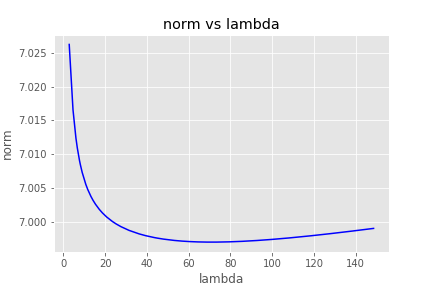
\includegraphics[scale = 0.54]{Images/norm_vs_lambda.png}
	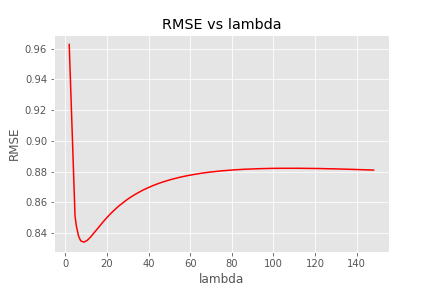
\includegraphics[scale = 0.54]{Images/RMSE_vs_lambda.png}
\end{enumerate}
\end{solution}
\newpage

\begin{problem}[3 (continued)]
\begin{enumerate}[(a)]
	\setcounter{enumi}{3}
\item (\textbf{math}) Consider regularized linear regression where we pull the
basis term out of the feature vectors. That is, instead of computing $\hat\yy
= \thetab^\T\xx$ with $\xx_0 = 1$, we compute $\hat\yy = \thetab^\T\xx + b$.
This corresponds to solving the optimization problem
\[
\text{minimize: } ||A\xx + b\1 - \yy||_2^2 + ||\Gamma\xx||_2^2.
\]
Solve for the optimal $\xx^\star$ explicitly. Use this close form to compute the
bias term for the previous problem (with the same regularization strategy). Make
sure it is the same.
\newline
\item (\textbf{implementation}) We can also compute the solution to the least squares
problem using gradient descent. Consider the same bias-relocated objective
\[
\text{minimize: } f = ||A\xx + b\1 - \yy||_2^2 + ||\Gamma\xx||_2^2.
\]
Compute the gradients and run gradient descent. Plot the $\ell_2$ norm
between the optimal $(\xx^\star, b^\star)$ vector you computed in closed form
and the iterates generated by gradient descent. Hint: your plot should move
down and to the left and approach zero as the number of iterations increases. If
it doesn't, try decreasing the learning rate.
\end{enumerate}
\end{problem}
\begin{solution}
	\begin{enumerate}[(d)]
	    \item We are trying to find a closed form solution to 
    	\[
        \text{minimize: } ||A\xx + b\1 - \yy||_2^2 + ||\Gamma\xx||_2^2.
	    \]
	    Letting $\mathbf{a_i}$ be the ith row vector of the matrix $A$ this is:
	    \[
	    \text{minimize: } (A\xx + b\1 - \yy)^T(A\xx + b\1 - \yy) + (\Gamma\xx)^T(\Gamma\xx)
	    \]
	    To do this we find the critical points by finding the gradient with respect to $\xx$ and $b$ and set to 0, but first lets expand:
	    \[
	    (A\xx + b\1 - \yy)^T(A\xx + b\1 - \yy) + (\Gamma\xx)^T(\Gamma\xx) = (\xx^TA^T + b\1^T - \yy^T)(A\xx + b\1 - \yy) + (\xx^T\Gamma^T)(\Gamma\xx)
	    \]
	    \[
	    = (\xx^TA^TA\xx + b\1^TA\xx + \xx^TA^Tb\1 + b\1^Tb\1 - \yy^TA\xx - \yy^Tb\1 - \xx^TA^T\yy - b\1^T\yy + \yy^T\yy +  \xx^T\Gamma^T\Gamma\xx)
	    \]
	    Taking the gradient of each term with respect to $b$ this will be 0:
	    \[
	    \1^TA\xx + \xx^TA^T\1 + 2\1^Tb\1 - \yy^T\1 - \1^T\yy = 0
	    \]
	    \[
	    2\1^Tb\1 = \yy^T\1 + \1^T\yy - \1^TA\xx - \xx^TA^T\1
	    \]
	    \[
	    b = \frac{\yy^T\1 + \1^T\yy - \1^TA\xx - \xx^TA^T\1}{2n}
	    \]
	    \[
	    b = \frac{\yy^T\1 - \xx^TA^T\1}{n}
	    \]
	    Taking the gradient of each term with respect to $\xx$ this will be 0:
	    \[
	    2A^TA\xx + A^Tb\1 + A^Tb\1 - A^T\yy - A^T\yy + 2\Gamma^T\Gamma\xx = 0
	    \]
	    \[
	    A^TA\xx + A^Tb\1 - A^T\yy + \Gamma^T\Gamma\xx = 0
	    \]
	    Now we plug in the optimal $b$ we found:
	    \[
	    A^TA\xx + \frac{\yy^T\1 - \xx^TA^T\1}{n}A^T\1 - A^T\yy + \Gamma^T\Gamma\xx = 0
	    \]
	    \[
	    nA^TA\xx + \yy^T\1A^T\1 - \xx^TA^T\1A^T\1 - nA^T\yy + n\Gamma^T\Gamma\xx = 0
	    \]
	    \[
	    nA^TA\xx - \1^TA\1^TA\xx + n\Gamma^T\Gamma\xx = nA^T\yy - \yy^T\1A^T\1
	    \]
	    \[
	    (nA^TA - \1^TA\1^TA + n\Gamma^T\Gamma)\xx = nA^T\yy - \yy^T\1A^T\1
	    \]
	    \[
	    \xx = (nA^TA - A^T\1\1^TA + n\Gamma^T\Gamma)^{-1}(nA^T\yy - \yy^T\1A^T\1)
	    \]
	    \textbf{Important note:} I had to copy most of the solution code for both (d) and (e) coding parts. After I attempted on my own for quite some time, I was out of time and using the solution code to figure out what was wrong with mine, because even though I think my solution to the math part of (d) is equivalent to the solution given, they are too different for me to use the code to fix my code.
	    
	    The code told me that:\newline
	    Difference in bias is  4.3279E-10\newline
        Difference in weights is  5.7041E-10
        
        \item The plot I obtained was the following:\newline
        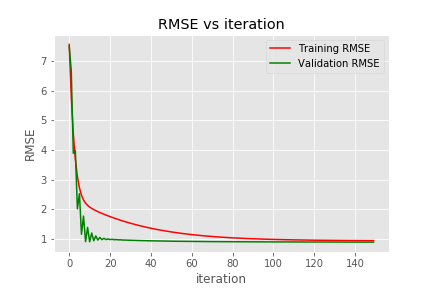
\includegraphics[scale = 0.7]{Images/convergence.png}\newline
        Difference in bias is  1.5387E-01 \newline
        Difference in weights is  7.9950E-01
	\end{enumerate}
\end{solution}
\newpage

\end{document}
